\documentclass{article}

\usepackage{listings}
\usepackage{color}
\usepackage{graphicx}
\usepackage{titlesec}
\usepackage{amsmath}
\usepackage{hyperref}
\usepackage{amsmath}
\definecolor{dkgreen}{rgb}{0,0.6,0}
\definecolor{gray}{rgb}{0.5,0.5,0.5}
\definecolor{mauve}{rgb}{0.58,0,0.82}

\lstset{frame=tb,
  language=Python,
  aboveskip=3mm,
  belowskip=3mm,
  showstringspaces=false,
  columns=flexible,
  basicstyle={\small\ttfamily},
  numbers=none,
  numberstyle=\tiny\color{gray},
  keywordstyle=\color{blue},
  commentstyle=\color{dkgreen},
  stringstyle=\color{mauve},
  breaklines=true,
  breakatwhitespace=true,
  tabsize=3
}

\newcommand{\inlinecode}[2]{{\lstinline[language=#1]$#2$}}

\begin{document}

\title{%
  \textbf{Banknote Authentication Design Considerations} \\
  \large Machine Learning for Security and  \\
    Performance in Production Settings}
\author{Alice Chang, Karthik Umashankar, Yu Chen}
\maketitle

\begin{abstract}
Banknote authentication is a high-value task within the financial services industry. In this paper, we perform a validation study and probe into potential vulnerabilities of online machine learning models utilized for this task. In particular, we utilize the work of  "Banknote Authentication" by Gillich and Lohweg\cite{original_paper}. The authors utilized an industry-standard technique of filtering the banknote grayscale image for viable regions of interest, and then performing a novel Shift Invariant Wavelet Transform for the model's feature engineering. We first validate Gillich and Lohweg's findings of 100\% accuracy on holdout datasets using a multitude of models (k-Nearest Neighbors, Support Vector Machine, etc.), and then identify critical thresholds where sample size begins to negative impact the potential performance of a machine learning model once deployed into production.
\newline\newline
We conclude by investigating potential vulnerabilities an online machine learning system can encounter, namely the Frog Boiling Attack. We outline a potential implementation of this type of penetration attack and highlight various potential countermeasures to mitigate its negative impact on a machine learning system in production.
\end{abstract}

\section{Introduction}
The Intaglio technique used within banknote printing allows for an unmatched sharpness in contrast through a feelable relief\cite{intaglio} .This technique forms a vital component of modern-day banknote authenticity verification. In the initial phase of authentication, \textbf{image digitization} occurs where the banknote's relief is captured through industry-grade cameras to produce an image grayscale that can be then undergo a feature transformation, such as the Wavelet Transform (WT). Prior to feature transformation, various \textbf{Regions of Interest (ROI)}.  Regions with low mean and variance in grayscale values of the various blocks are selected:
\begin{figure}
  \caption{A scatter plot from Gillich and Lohweg, 2010 showing the decision boundaries for selection of viable regions of interest. The circles are classified as appropriate ROIs while the squares are discarded for non-homogeneity or high mean grayscale values.}
  \centering
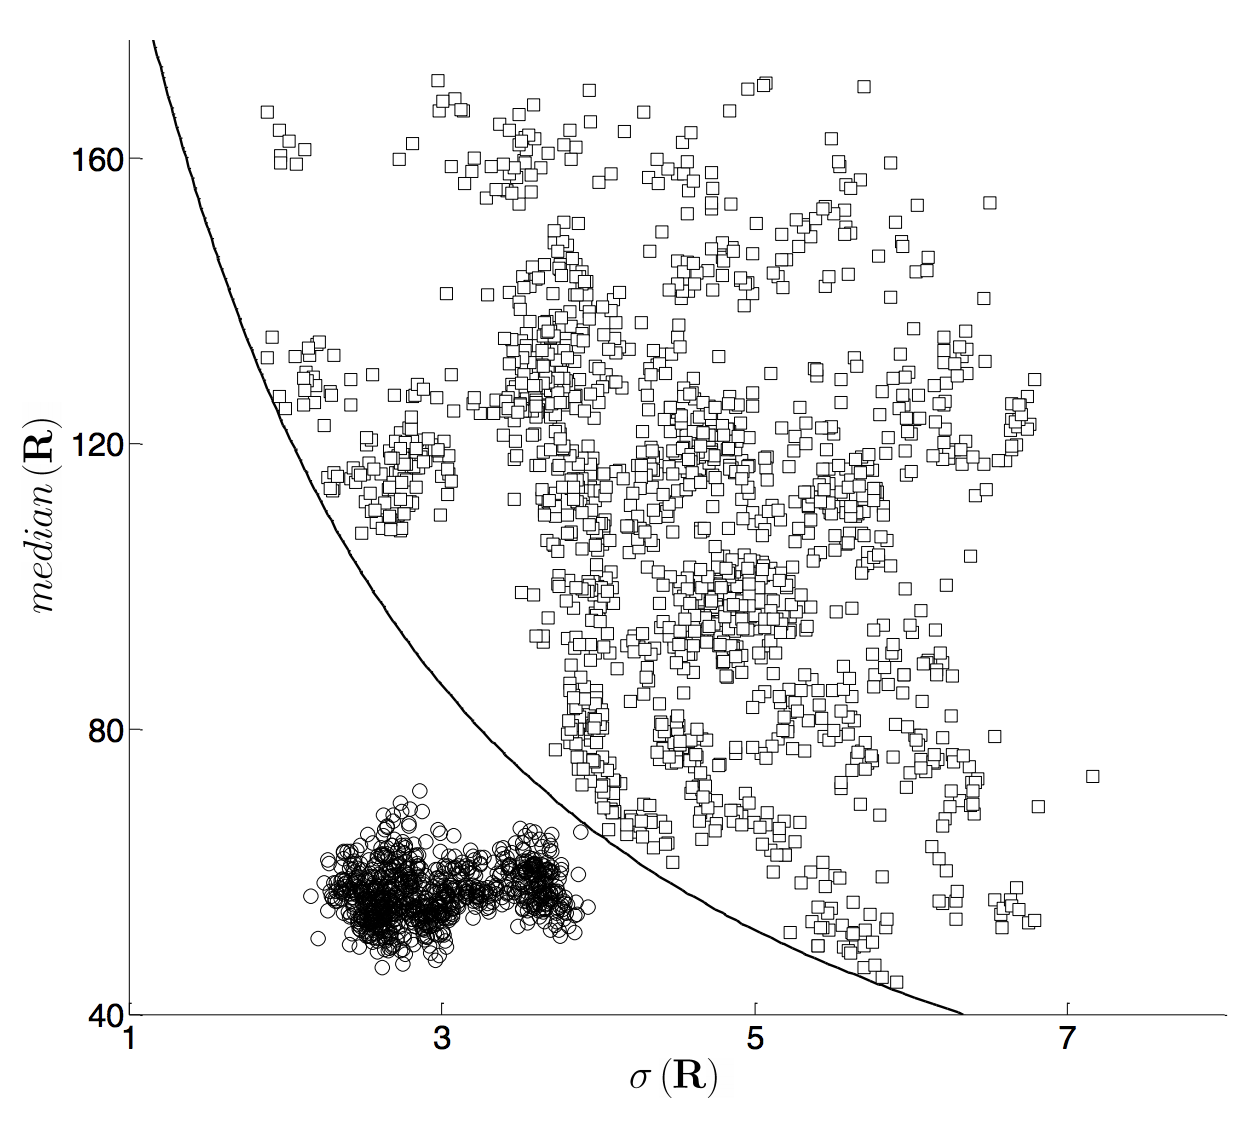
\includegraphics[width=100mm]{roi_selection.png}
\end{figure}
\section{Related Work}

\section{Experiments}

\subsection{Validation of Model Performances}
In their original paper, Gillich and Lohweg assert that 100\% accuracy can be achieved as a result of judicious Region of Interest selection and the Shift Invariant Transform. To validate, we performed basic data processing, scaling the dataset so that each feature column $k$ had $\mu_{k} = 0$ and a $\sigma_{k} = 1$:

\begin{lstlisting}
import pandas as pd
import numpy as np
from sklearn.model_selection import train_test_split
from sklearn.preprocessing import StandardScaler

df = pd.read_csv("data/dataset.csv", encoding="latin-1") # import the CSV dataset and save as a Pandas dataframe object
    
targets = df["class"].values # save the targets (Y) as a NumPy array of integers
features_df = df.loc[:, df.columns != "class"] # save everything else as the features (X)
    
features_names = features_df.columns.values # save the column names
features_matrix = features_df.values # convert X from a dataframe to a matrix (for our machine learning models)
scaled_features_matrix = StandardScaler().fit_transform(features_matrix) # scale the data so mean = 0, unit variance - important for many models
\end{lstlisting}

The cleaned \lstinline{scaled_features_matrix} Numpy object can then be fed into a variety of different models:

\begin{lstlisting}
logistic_regression = LogisticRegression()
logistic_regression.fit(X_train, y_train)
training_predictions = logistic_regression.predict(X_train)
test_predictions = logistic_regression.predict(X_test)

# check accuracy of Logistic Regression
number_correct = np.sum(training_predictions == y_train)
number_correct_test = np.sum(test_predictions == y_test)
\end{lstlisting}

\subsection{Sample Size Stress Testing}

\subsection{Implementation of Frog Boiling Attack (FBA)}

The Frog Boiling Attack is most effective during business contexts where online learning occurs (when data arrives as a stream and becomes ingested sequentially, with the fitted model updated after each new data point). The attack relies upon the concept of template drift\cite{template_drift}, where the model's fitted "template" of an authentic banknote data sample is corrupted over time by a stream of compromised data points. The overall implementation, implemented over $N$ steps, relies upon the update equation

\begin{equation}
F_{new} = F_{old} + (i - 1)\delta(x)
\end{equation}

where

\begin{equation}
\delta(x) = \frac{\bar{x}_{target}-\bar{x}_{original}}{N}
\end{equation}

\subsubsection{FBA Countermeasures}

\begin{itemize}
  \item \textbf{Freezing Online Learning}: When discussing potential countermeasures to FBA, a tradeoff between responsiveness and security must be established. An obvious, yet sometimes unrealistic, method of prevention is to fully disable online learning completely, and "freeze" the authentication classifier. In many businesses cases, disabling online learning may result in a significant decline in model performance, especially if the feature space is exceptionally dynamic (ie. consumer entertainment and purchasing behavior, which is often a function of seasonality and inherent "drift").
  \item \textbf{Autocorrelation Detection}: An "honest" user (one who is utilizing the business' services as intended) should display no correlation between her submitted banknote data points. No correlation between a user's data points over time equates to each banknote being submitted independently of the prior banknotes (which should be the case if no fraudulent activity is happening).
  \item \textbf{Batch Model Updates}: The crux of the Frog Boiling Attack is the assumption that the model will not be able to detect small "drift" towards a target template, capitalizing upon the inherent responsiveness of the model towards new data points. However, batching model updates increases the magnitude of "drift", with the hope being that the model is able to successfully detect larger "steps" if we perform model updates in batches. The pseudocode implementation for batching would be as follows:
\begin{lstlisting}
for user in users:
	BATCH_SIZE = 30 # update after user has submitted 30 banknotes
	batched_datapoints = [] # create a cache of datapoints per user
	authenticated = receive_data(banknote_datapoint) # ingest datapoint when user submits banknote
	
	if banknote_datapoint is authenticated:
		batched_datapoints.append(banknote_datapoint)
	else:
		batched_datapoints = [] # if any authentication points fail, clear the cache
		
	if length(batched_datapoints) == BATCH_SIZE: # once cache hits batch size, update the global model
		update_model(batched_datapoints)
\end{lstlisting}
Within this particular implementation, a key hyperparameter to optimize is \lstinline!BATCH_SIZE! This is the number of drift steps taken from the original template to the target template \textit{without updates (ie. model refitting)} before the model returns a negative classification. For instance, in our implementation of frog boiling attack, disabling the online learning model refitting and thereby freezing the model, we receive the following log output:
\begin{verbatim}
Closest positive point: [ 0.13 0.01 -0.54  0.24]
Negative centroid: [ 0.65  0.40 -0.14 0.02]
Distance from negative centroid:  0.79
Prediction: [0]
Classified as negative during iteration 10
\end{verbatim}
The simple k-Nearest Neighbors model will accept drift up to 10 steps away before it detects a fraudulent banknote datapoints. Thus, we'd likely set our \lstinline!BATCH_SIZE! to a number significantly higher than 10. This number can be set by repeatedly probing the authentication model with online learning disabled to generate a distribution of \textbf{tolerance thresholds}, or the number of steps taken before the machine learning begins to classify data points as negative. Say we have taken 50 different probes of our model, and the following array of tolerance thresholds are returned:

\begin{verbatim}
[ 7.,  4.,  2.,  9., 13.,  9., 10.,  9., 13.,  8.,  8., 14.,  8.,
10.,  3., 12.,  9., 15., 12.,  8.,  8., 13., 10.,  5.,  8., 15.,
6., 14.,  8.,  8., 15.,  6.,  6.,  6., 15.,  5., 11., 10.,  9.,
13., 10., 13.,  7.,  9.,  8., 11., 15.,  8., 10., 16.]
\end{verbatim}

We can fit these results to a Gaussian distribution, and then find its inverse cumulative distribution function (ICDF) at an acceptable $\alpha$ level. In the context of banknote authentication, given the sensitive nature of financial assets at risk, a relatively stringent $\alpha$ can be selected of 0.001:
\begin{lstlisting}
from scipy.stats import norm
alpha = 0.001
fitted_mean = 10
fitted_standard_deviation=3
threshold = int(norm.ppf(1-alpha, loc=fitted_mean, scale=fitted_standard_deviation))
print(f"Batch size at alpha level {alpha} is {threshold}")
# Batch size at alpha level 0.001 is 17
\end{lstlisting}

Thus, a \lstinline!BATCH_SIZE! of 17 is selected for production deployment to minimize the risk of online learning intrusion attacks like FBA.

 \end{itemize}

\subsubsection{FBA Optimizations}

\begin{itemize}
\item \textbf{Markov Chain Monte Carlo / Metropolis-Hastings Algorithm}:
\end{itemize}

\section{Future Work}

\begin{thebibliography}{9}
\bibitem{original_paper}
Eugen Gillich and Volker Lohweg. \textit{Banknote Authentication}. inIT - Institute Industrial IT, Department of Electrical Engineering and Computer Science, Ostwestfalen-Lippe University of Applied Sciences
November 2010
\bibitem{intaglio}
Van Renesse, R.L.: Optical Document Security, 3rd edn., Artehouse Boston/London
(2005)
\bibitem{template_drift} Z. Wang, A. Serwadda, K.Balagani, and Vir V. Phoha, "Transforming animals in a Cyber-Behavioral Biometric Menagerie with Frog-Boiling Attacks" in \textit{The IEEE Fifth International Conference on Biometrics: Theory, Application and Systems (BTAS 2012)}, Washington DC, 2012
\end{thebibliography}









\end{document}